\documentclass{article}
\usepackage[utf8]{inputenc}
\usepackage{graphicx}
\graphicspath{ {images/} }
\usepackage[usenames, dvipsnames]{color}
\usepackage[pagestyles]{titlesec}
\usepackage{atbegshi}% http://ctan.org/pkg/atbegshi
\AtBeginDocument{\AtBeginShipoutNext{\AtBeginShipoutDiscard}}

\definecolor{gray}{gray}{0.25}
\title{\color{white}ESCAPE: Game Manual}
\author{\color{white}Su Gao, Yuan Gao, James Lee, James Zhu }
\date{\color{white}9 April 2017}
\setlength{\footskip}{75pt}
\newpagestyle{main}{\color{white}\setfoot{}{}{\thepage}}
\pagestyle{main}
\assignpagestyle{\chapter}{main}
\color{white}

\begin{document}

\makeatletter
    \begin{titlepage}
        \begin{center}
            \begin{center}
            \pagenumbering{gobble}
            \makebox[\textwidth]{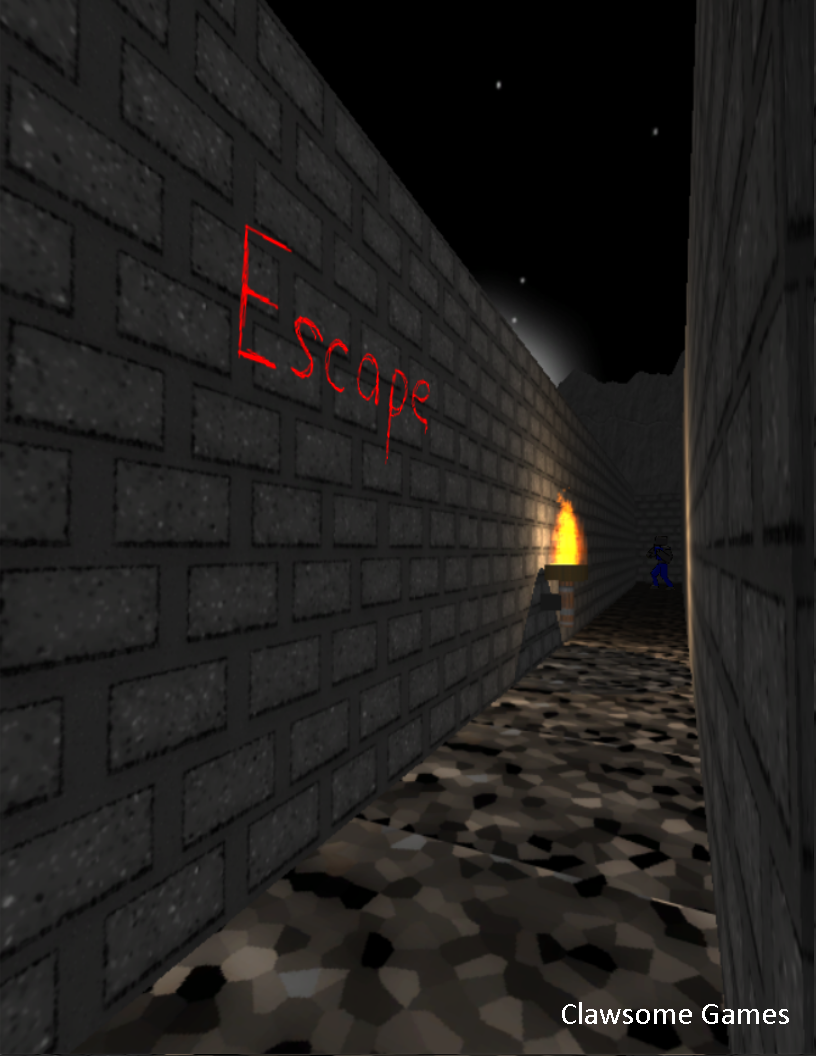
\includegraphics[trim = 0 0 0 167, width=\paperwidth]{title.png}}
            \end{center}
        \end{center}
    \end{titlepage}
\makeatother
\pagenumbering{arabic}
\maketitle
\pagecolor{gray}
\newpage
\color{white}
\tableofcontents

\section{Introduction}
\begin{center}
  \makebox[\textwidth]{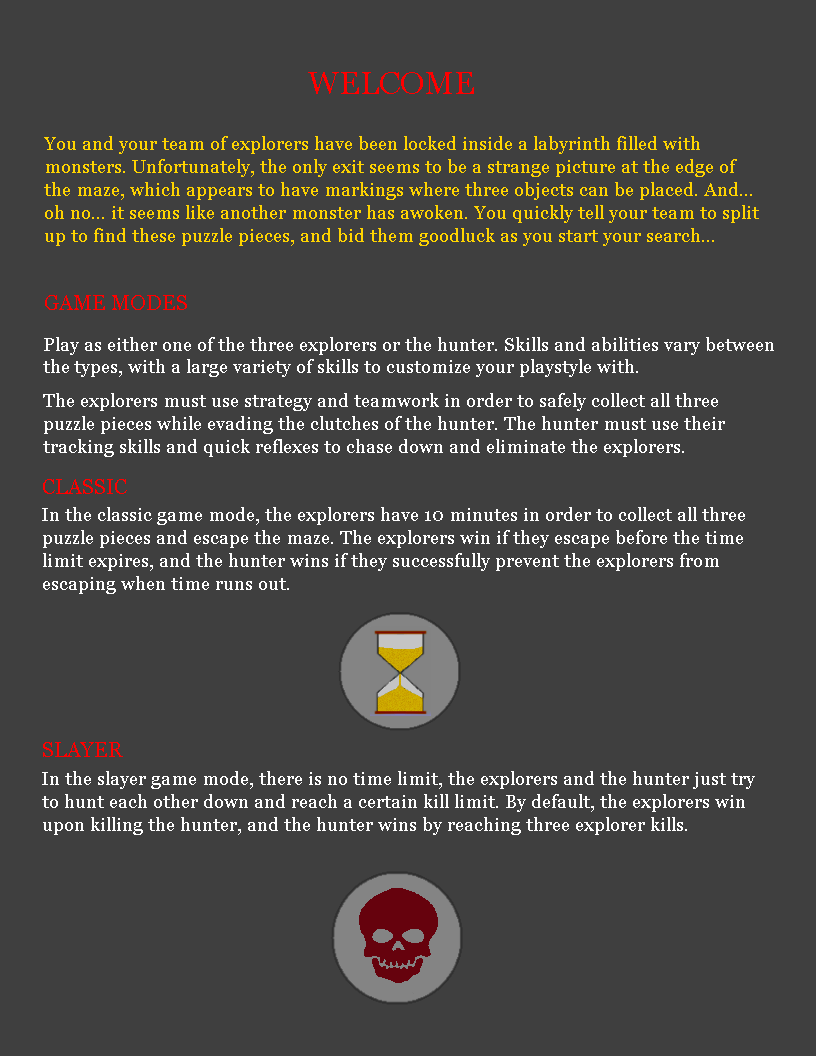
\includegraphics[trim = 0 0 0 200, width=\paperwidth]{Intro.png}}

\section{Getting Started}
\subsection{System Requirements}

    \makebox[\textwidth]{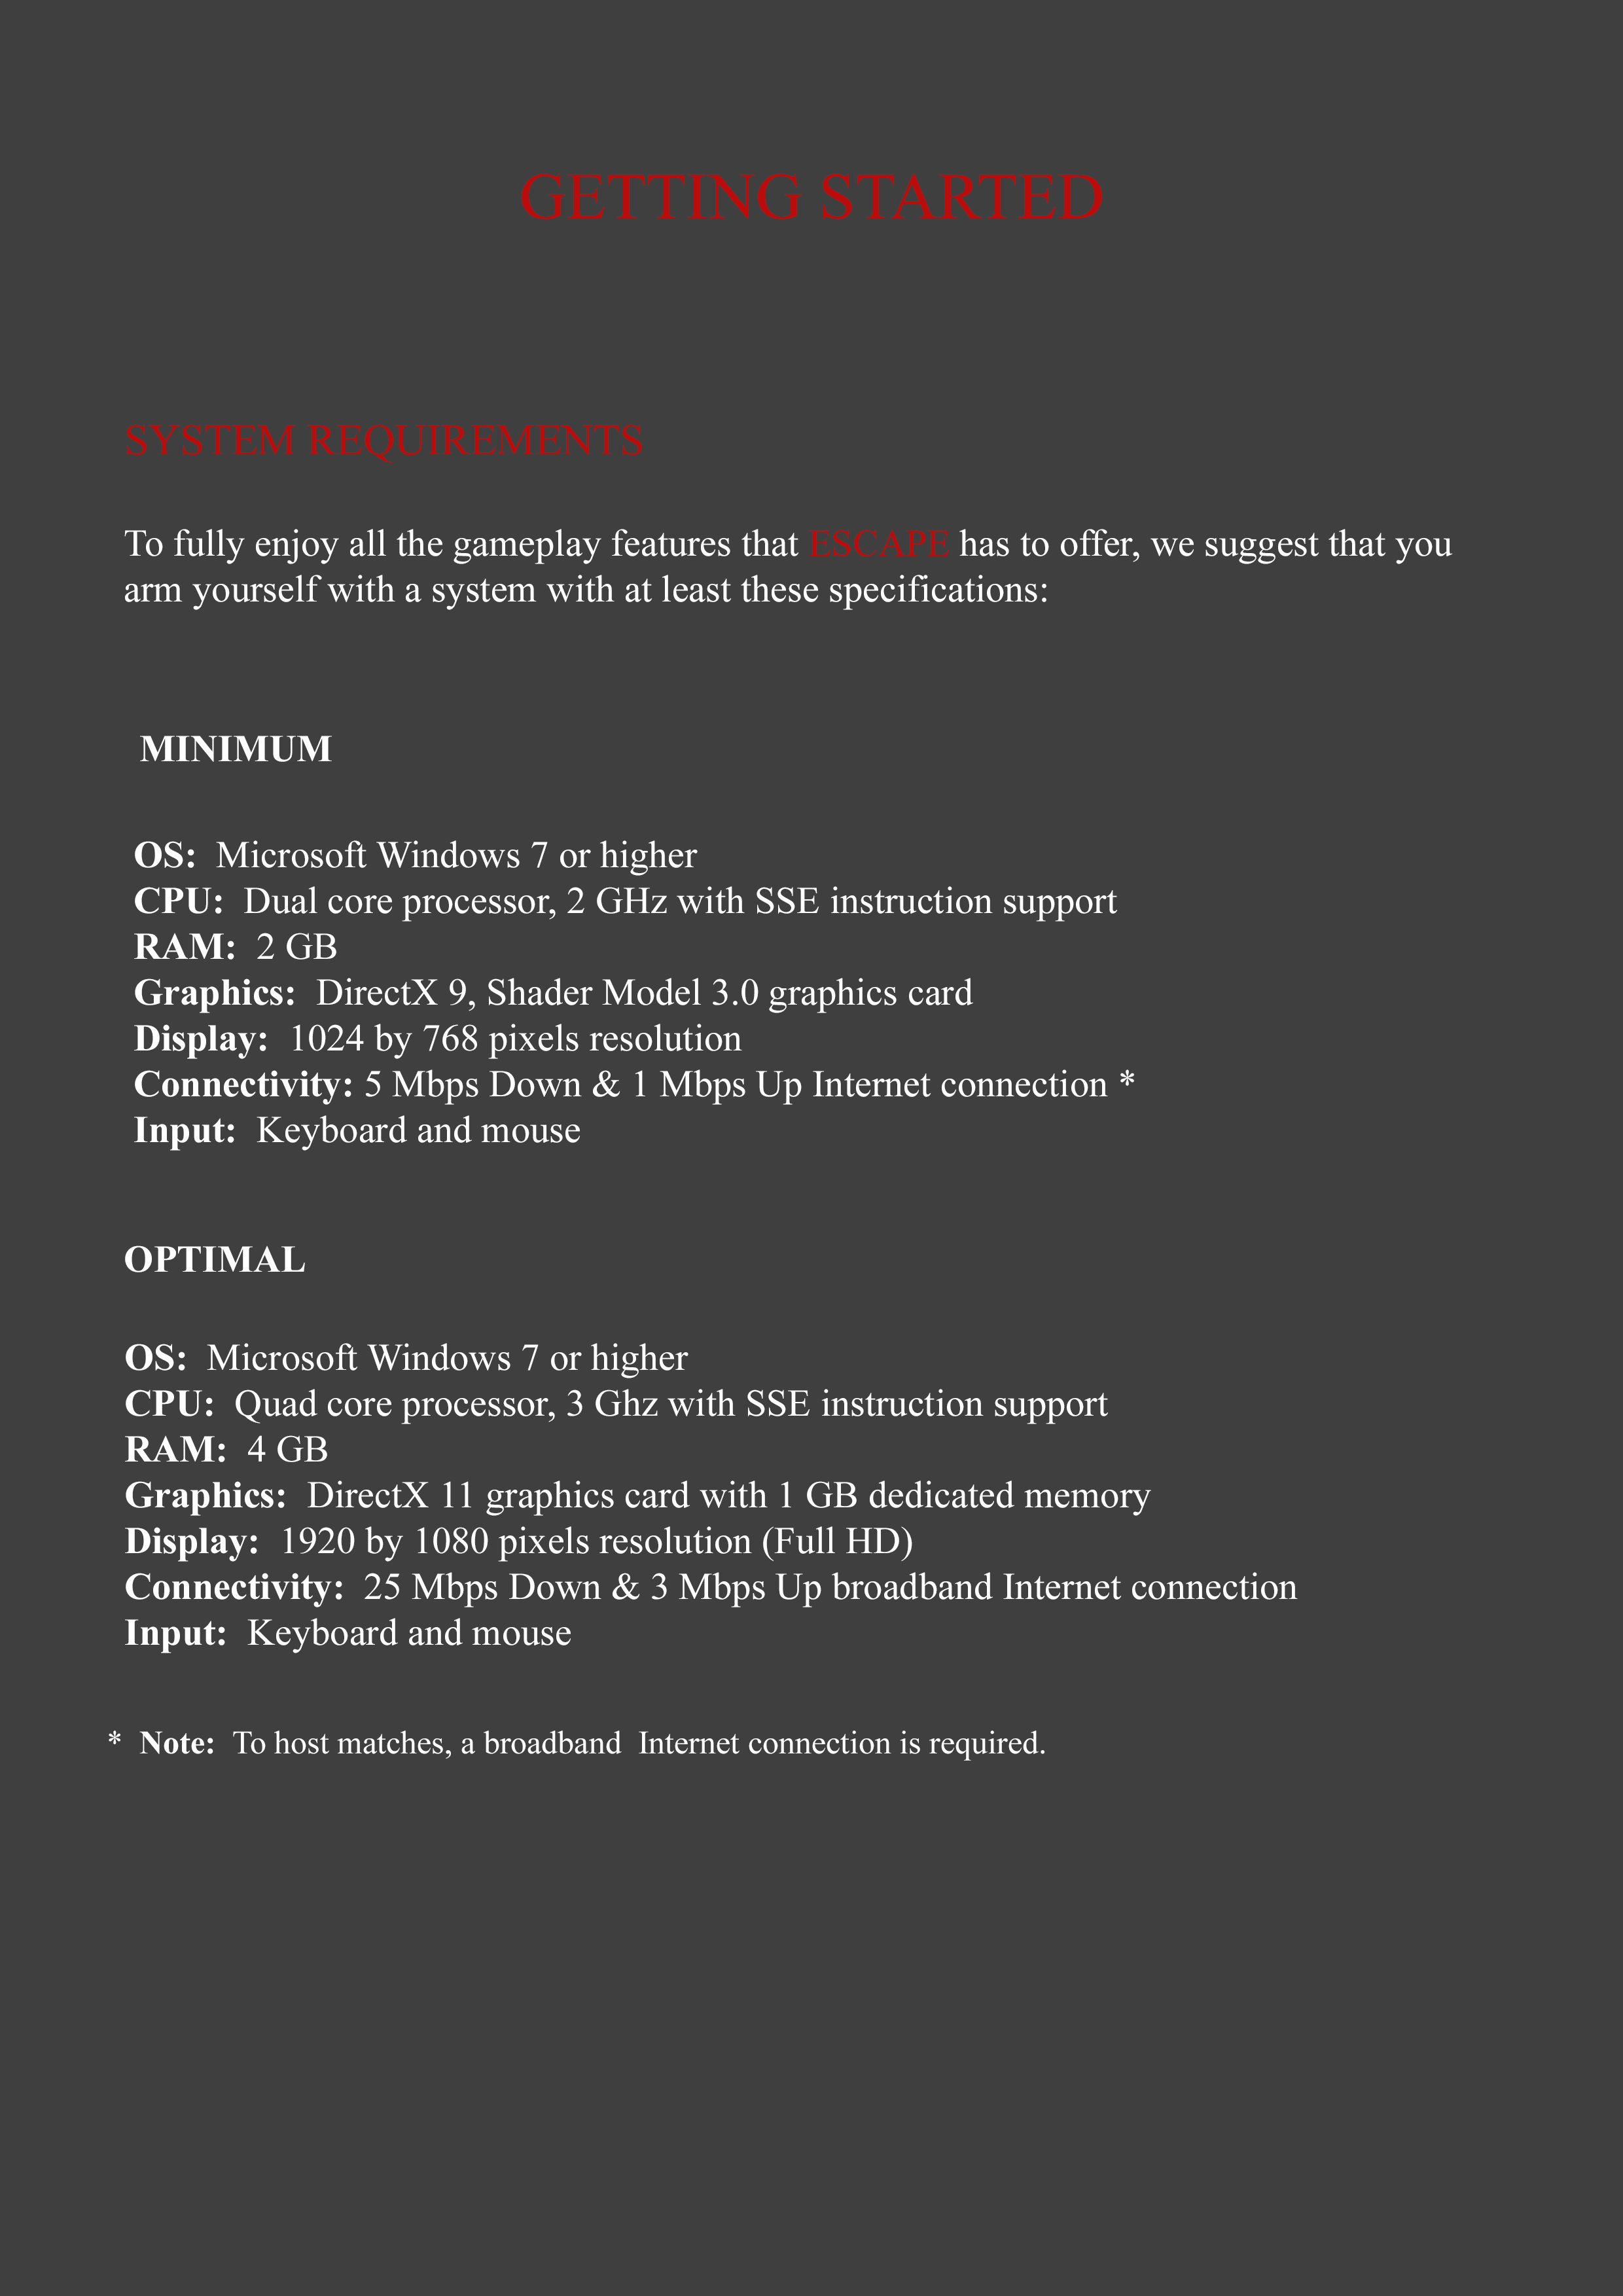
\includegraphics[trim = 0 0 0 165, width=\paperwidth]{gstarted-sys-req.png}}
    
\subsection{How to Install}

  \makebox[\textwidth]{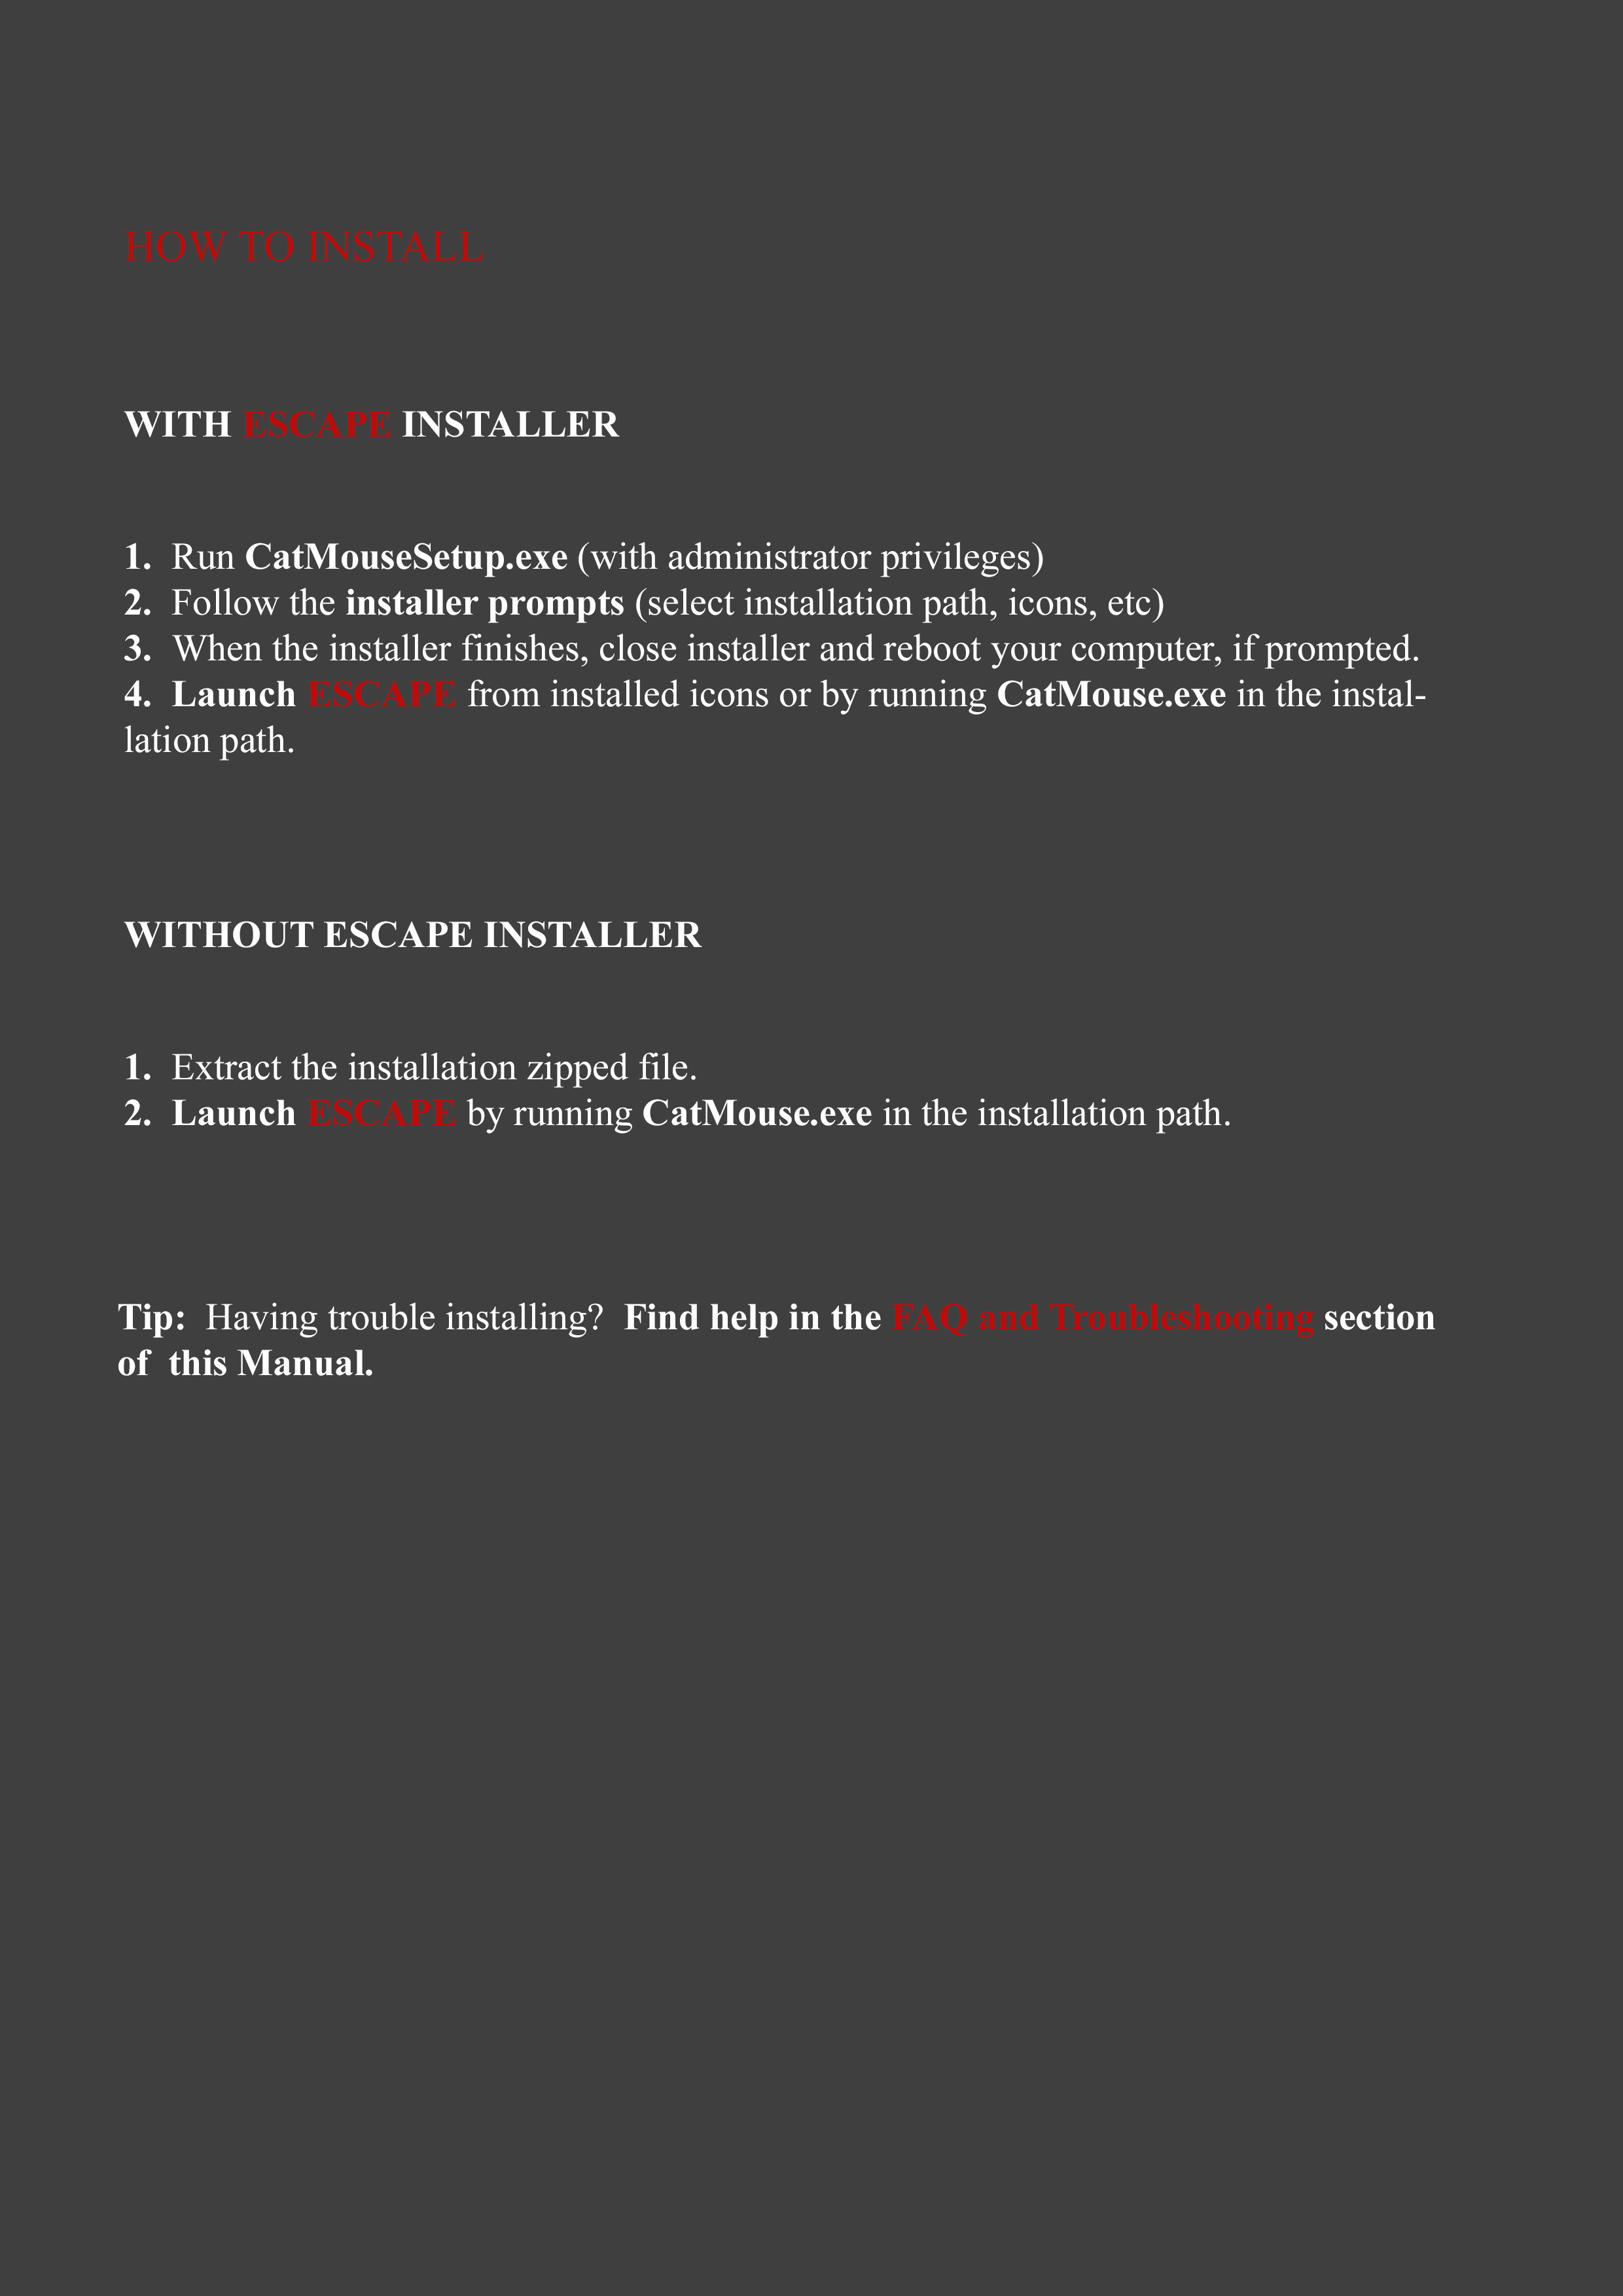
\includegraphics[trim = 0 0 0 165, width=\paperwidth]{gstarted-how-to-install.png}}

\section{How to Play}
\subsection{Controls}

  \makebox[\textwidth]{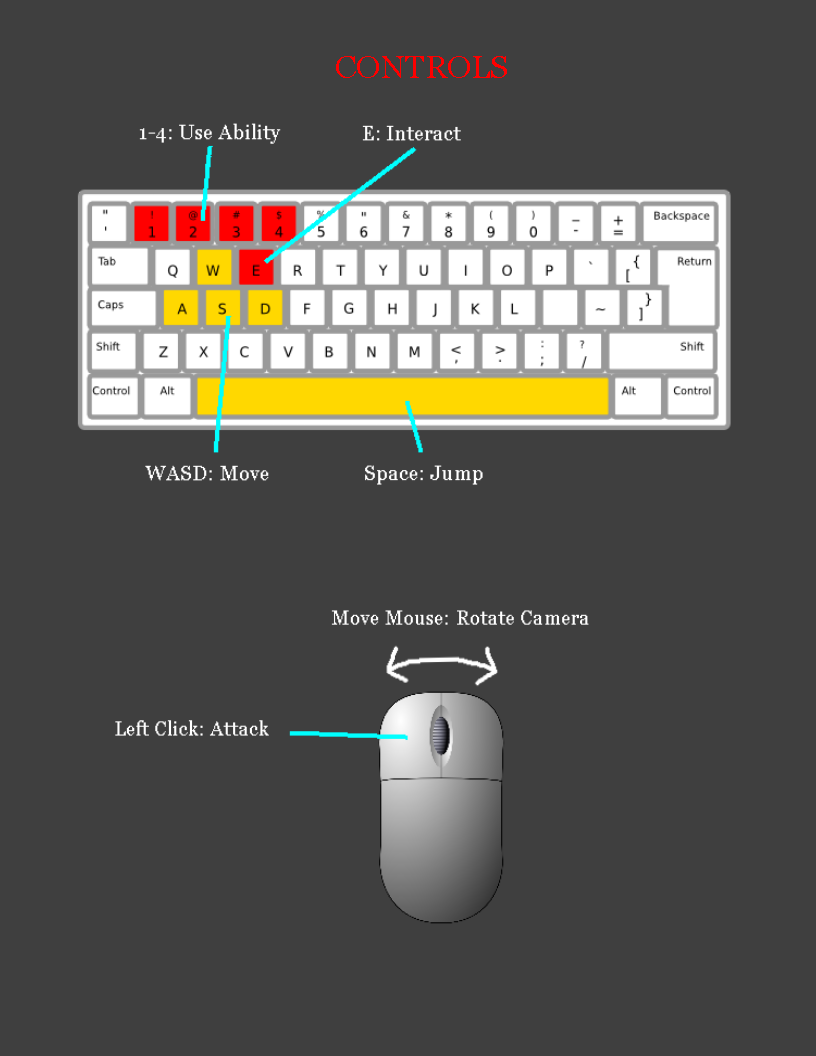
\includegraphics[trim = 0 0 0 250, width=\paperwidth]{Controls.png}}

\subsection{Interface}

  \makebox[\textwidth]{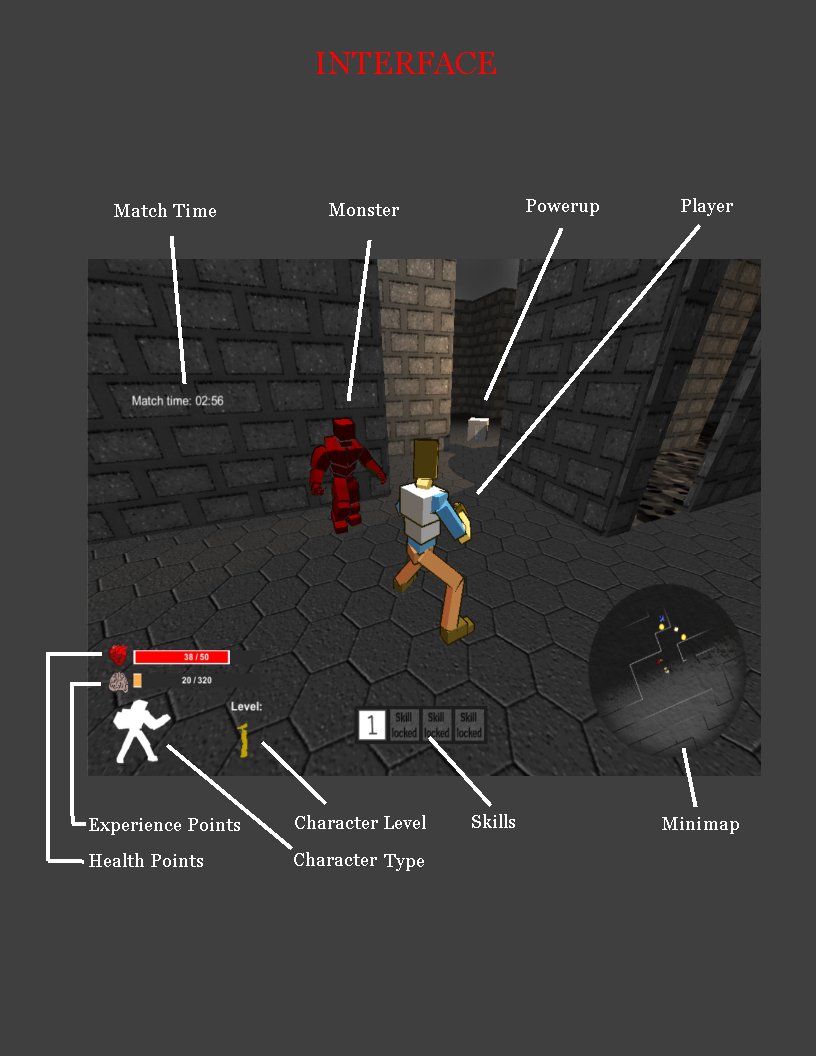
\includegraphics[trim = 0 0 0 165, width=\paperwidth]{interface.png}}

\subsection{Menus}

  \makebox[\textwidth]{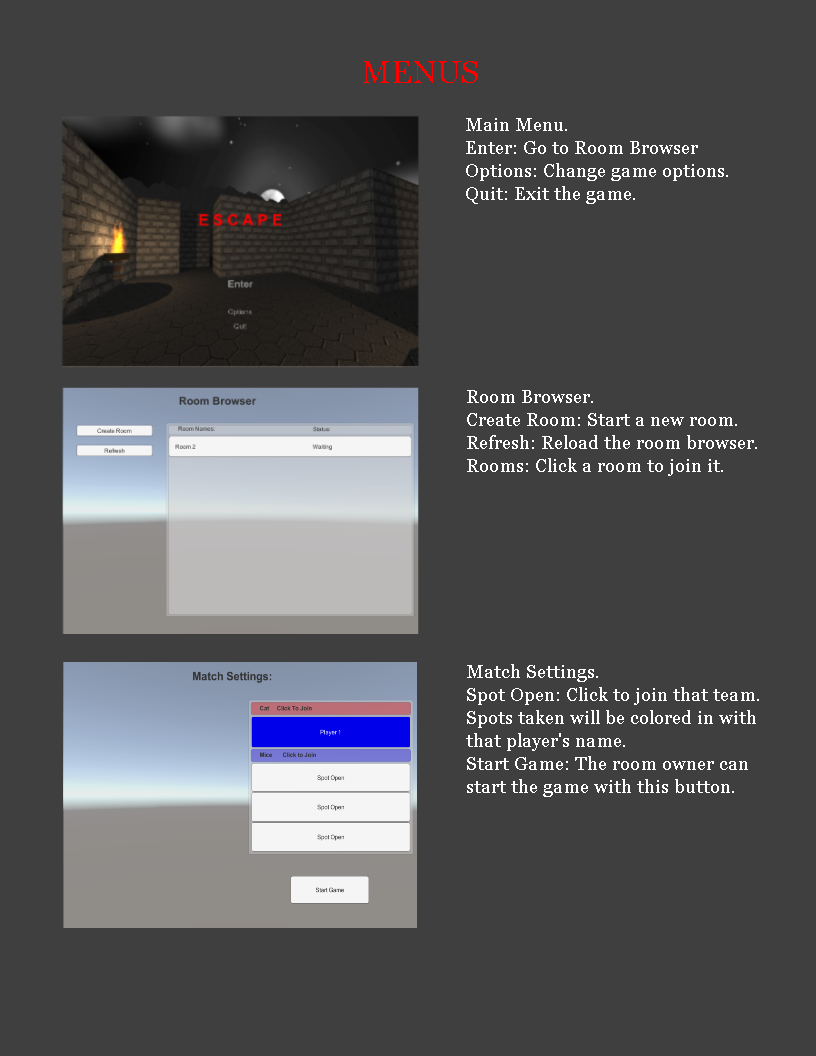
\includegraphics[trim = 0 0 0 165, width=\paperwidth]{menu.png}}

\subsection{Items and Skills}

  \makebox[\textwidth]{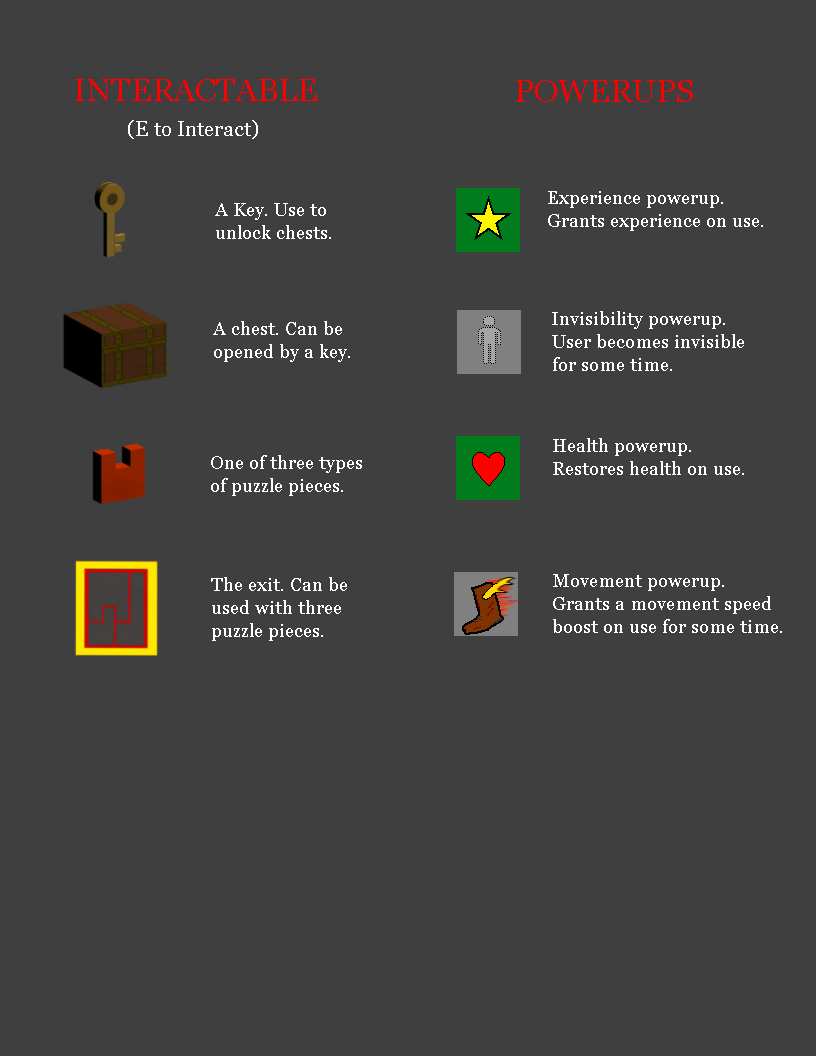
\includegraphics[trim = 0 0 0 165, width=\paperwidth]{itemsandskills.png}}

\subsection{Characters and Enemies}

  \makebox[\textwidth]{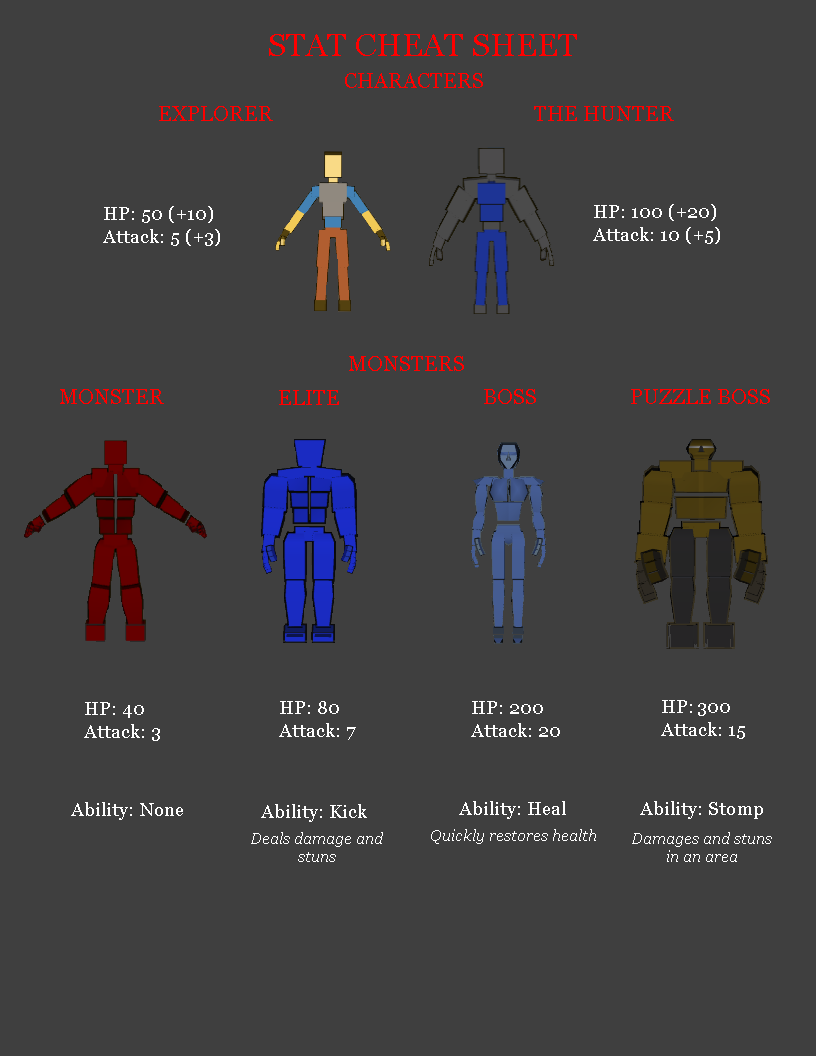
\includegraphics[trim = 0 0 0 165, width=\paperwidth]{CharStats.png}}
  
\section{FAQ and Troubleshooting}

  \makebox[\textwidth]{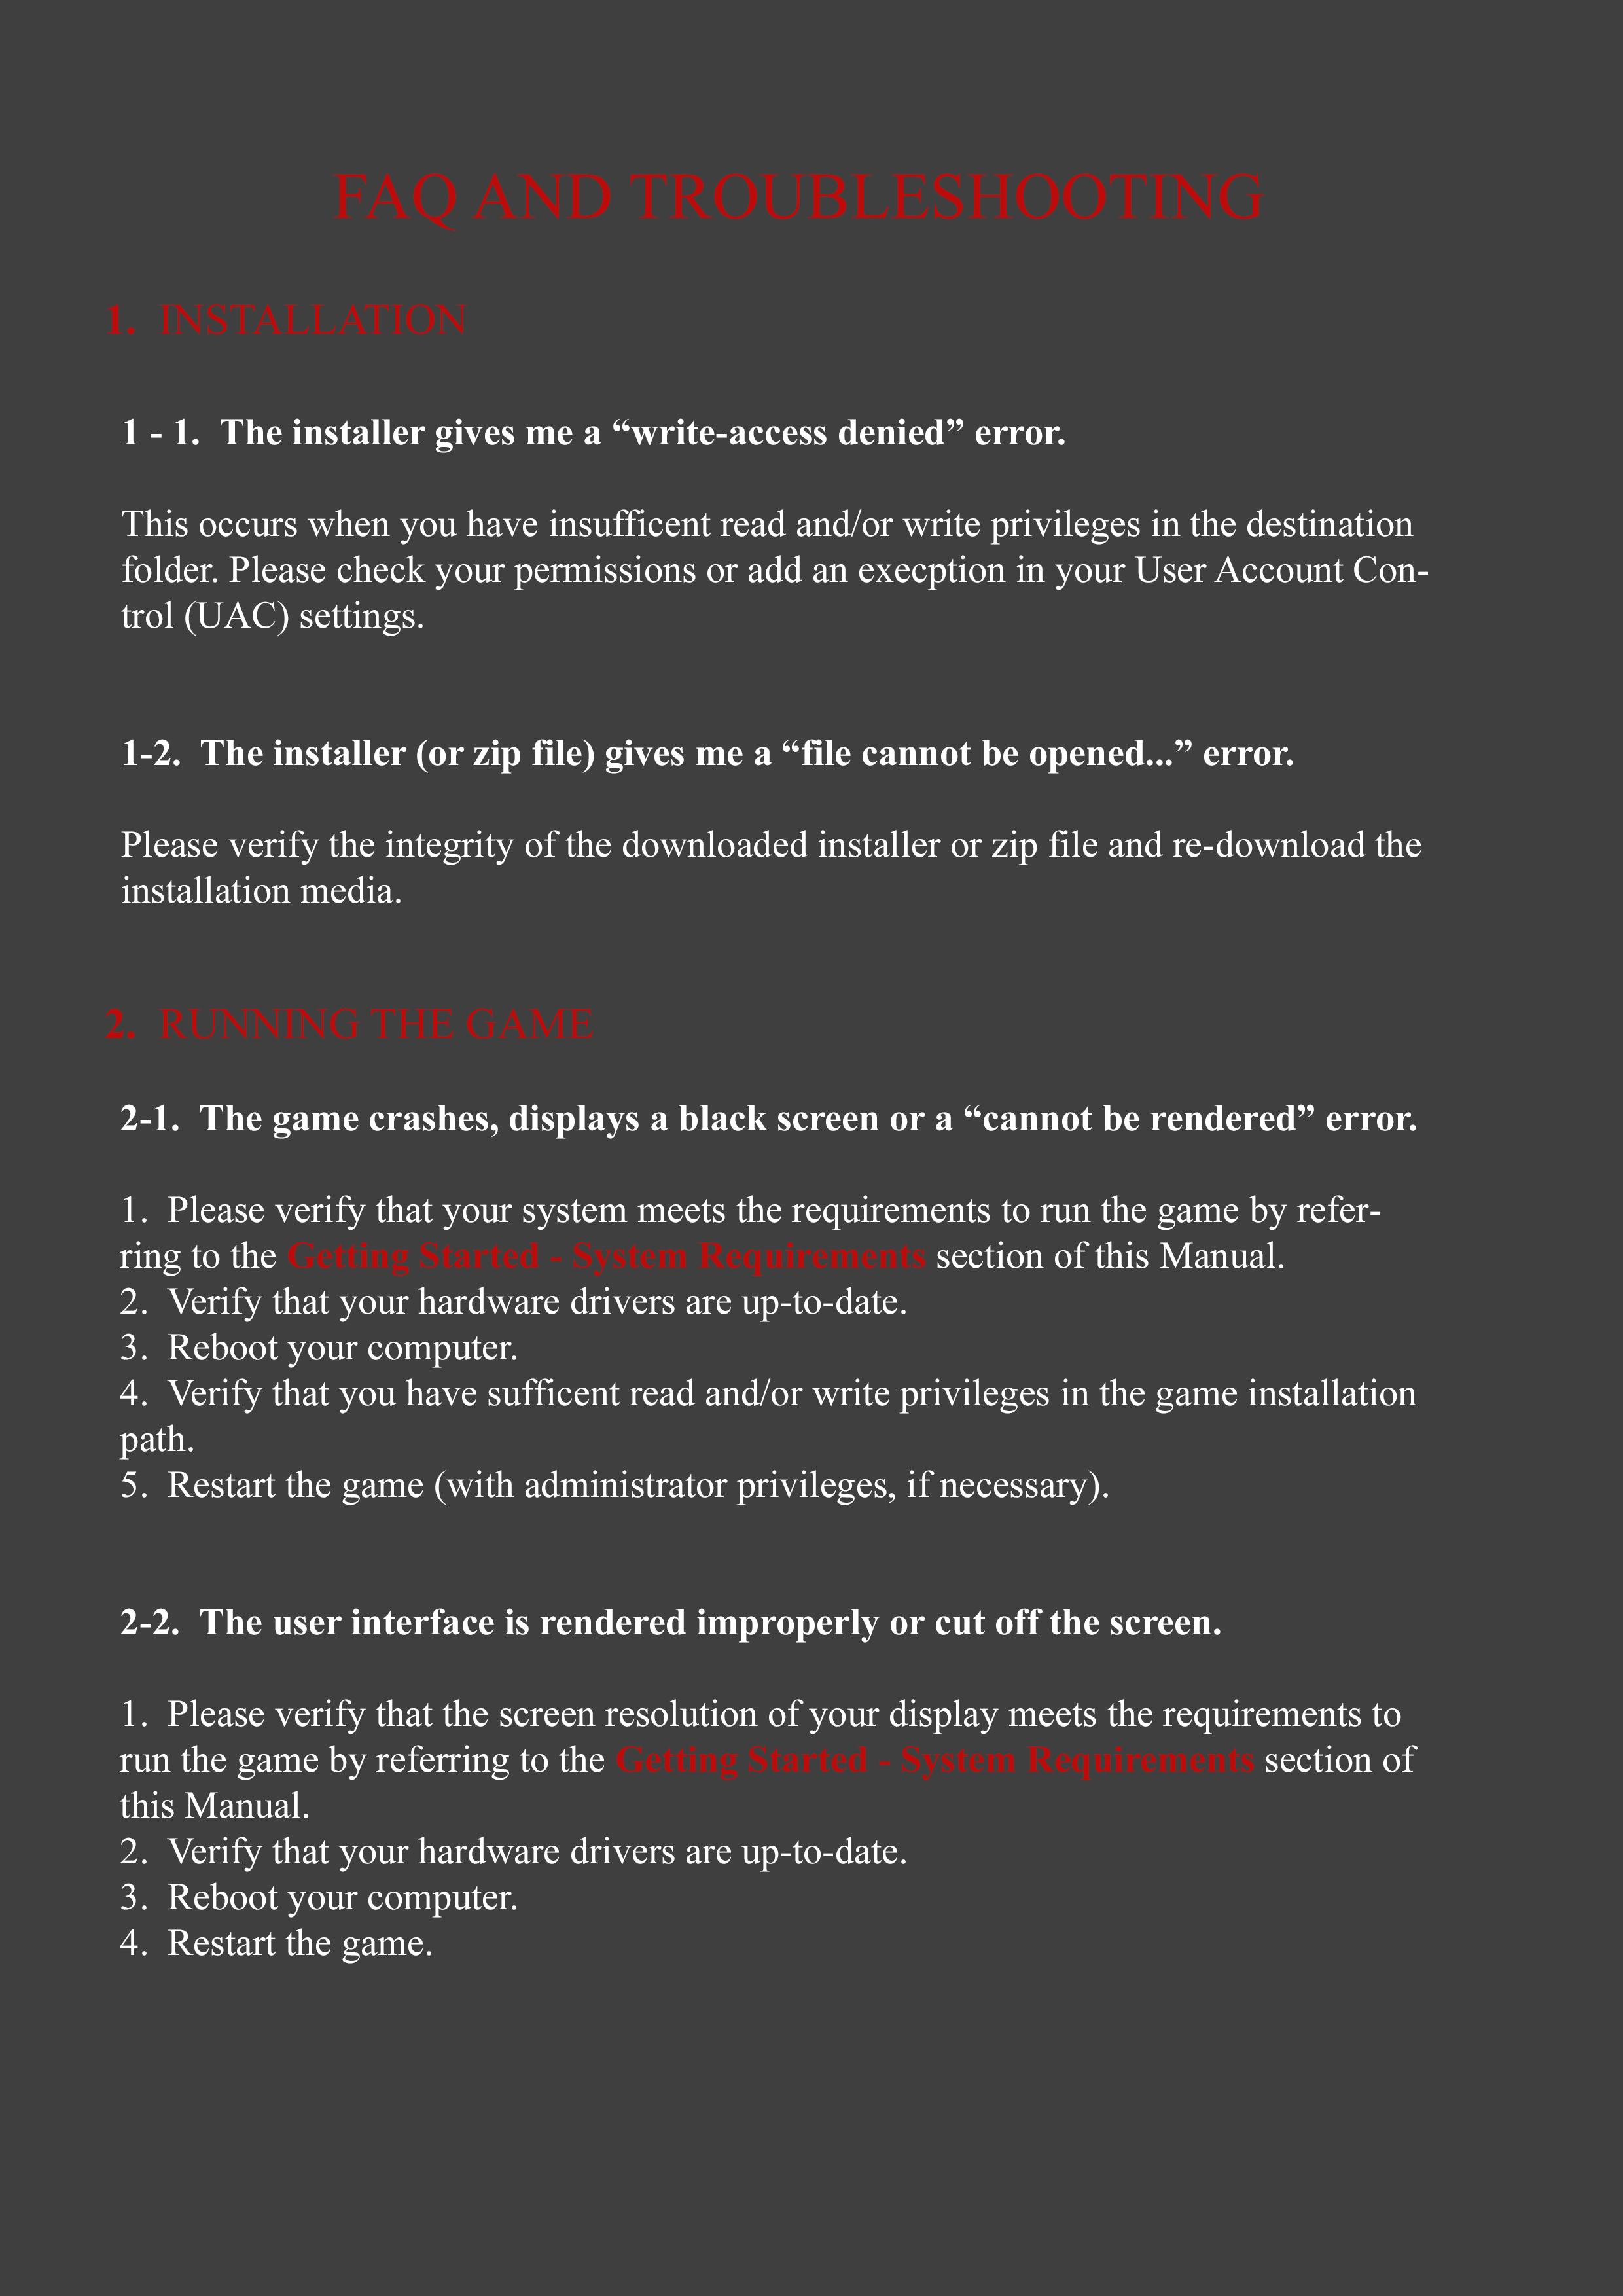
\includegraphics[trim = 0 0 0 165, width=\paperwidth]{faq-page-1.png}}
  \newpage 
  \makebox[\textwidth]{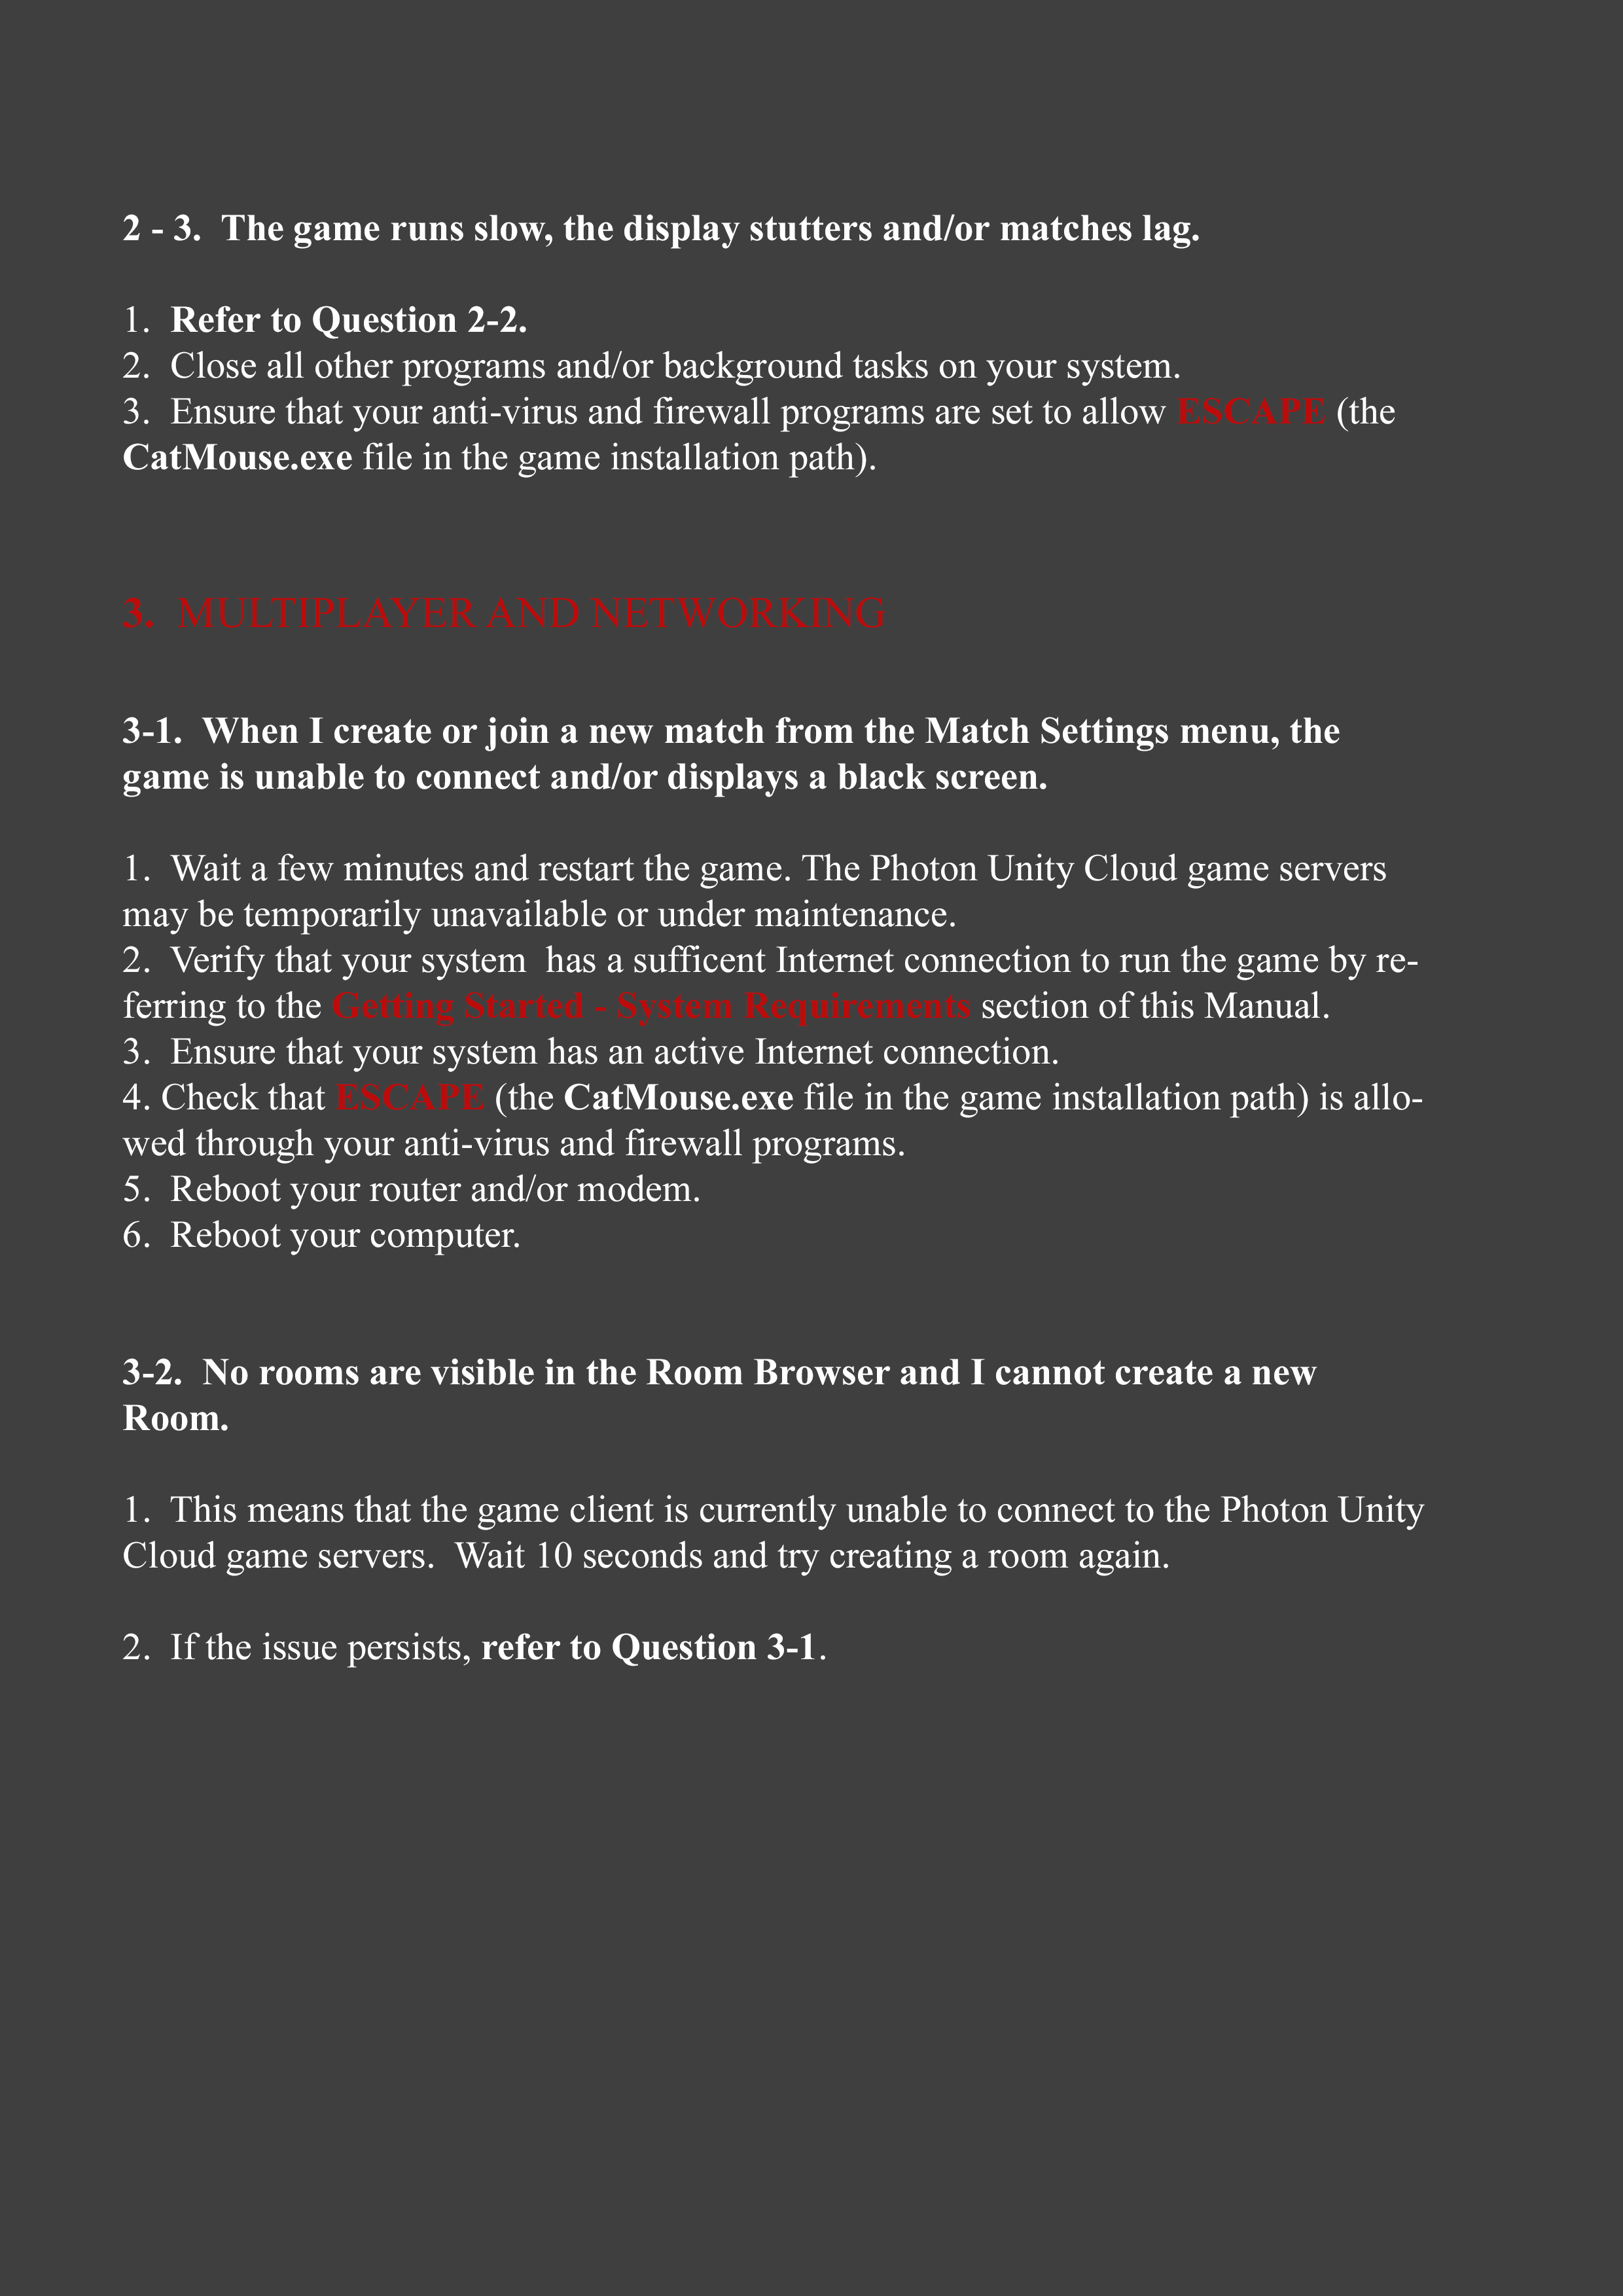
\includegraphics[trim = 0 0 0 165, width=\paperwidth]{faq-page-2.png}}

\section{Credits}

  \makebox[\textwidth]{
\includegraphics[trim = 0 0 0 165, width=\paperwidth]{credits.png}}
\end{center}
\end{document}